\documentclass[12pt]{article}
\usepackage{amsmath,amssymb}
\usepackage{color}
\usepackage{enumitem}
\usepackage{hyperref}
\usepackage{listings}
\usepackage{graphicx}

\lstset{
  basicstyle=\ttfamily,
  mathescape
}

% MAKE TITLE AND AUTHOR
\title{Natural language processing}
\author{
    Andrea Auletta
    \and
    Aulo
}

\date{\today}
\makeindex
\begin{document}
\maketitle
\tableofcontents
\newpage


\section{Text summarization with pretrained encoders}
\subsection{Some definitions}
\begin{itemize}
    \item \textbf{Good summary}: A good summary must be fluent and consistent, capture all the important topics, but not contain repetitions 
    of the same information;
    \item \textbf{Abstractive modeling}: the task requires language generation capabilities in order to create 
    summaries containing novel words and phrases not featured in the source text;
    \item \textbf{Extractive summarization}: is often defined as a binary classification task with labels 
    indicating whether a text span (typically a sentence) should be included in the summary;
    \item \textbf{Pretrained language model}: extends the idea of word embeddings by learning representations
    from large-scale corpora using a language modeling objective.
\end{itemize}
\subsection{Summary}
Here they explore the potential of Bert under a general framework encompassing both extractive 
and abstractive summarization. They combine the Pretrained Bert with a randomly-initialized Transformer 
decoder. The difference here is that we eant to manipulate multi-sentential input w.r.t. the usual task of Bert.
In Bert for summarization the document representations are learned hierarchically where lower transformer layers
represent adjacent sentences, while higher layers (+self-attention) represent multi-sentence discourse.
\begin{center}
    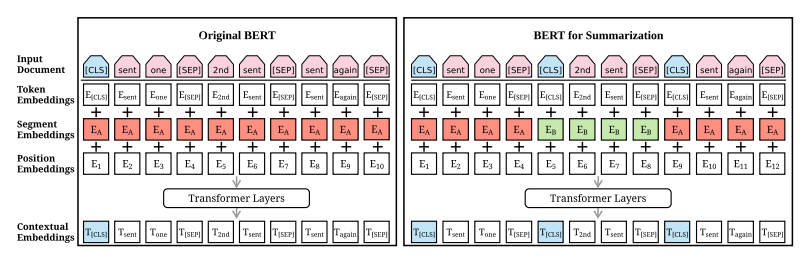
\includegraphics[scale=0.6]{./img/bert.png}
\end{center}
\subsubsection{Extractive summarization}
With BertSum we have the vector $v_i$ of the i-th [CLS] symbol from the top layer can be used as the 
representation of the i-th sentence. After this we have other inter-sentence transformer layers 
to capture document-level featurs for extracting summaries. The output layer is a sigmoid classifier.
\subsubsection{Abstractive summarization}
Standard encoder-decoder framework is used. The encoder is BertSum and the decoder is a 6-layered Transformer
initialized randomly. 
To circumvent the fact that the decoder is not pretrained is designed a new fine-tuning method: Adam 
optimizer with $\beta_1=0.9$ and $\beta_2=0.999$ for the encoder and the decoder, each with different
warmup-step and learning rates: 
\begin{itemize}
    \item $lr_\epsilon = \tilde{lr}_\epsilon \cdot min(step^{-0.5}, step \cdot warmup_\epsilon^{-1.5})$, 
    where $\tilde{lr}_\epsilon=2e^{-3}$, $warmup_\epsilon=20000$ for the encoder;
    \item $lr_\mathcal{D} = \tilde{lr}_\mathcal{D} \cdot min(step^{-0.5}, step \cdot warmup_\mathcal{D}^{-1.5})$, 
    where $\tilde{lr}_\mathcal{D}=0.1$, $warmup_\mathcal{D}=10000$ for the decoder;
\end{itemize}
The encoder can be trained with more accurate gradients when the decoder is becoming stable.
\subsection{implementation}
\begin{itemize}
    \item PyTorch;
    \item OpenNMT;
    \item bert-based-uncased: https://git.io/fhbJQ; 
    \item dropout for abstractive models;
    \item rouge-2 score for extractive models against gold summary (selct the top 3 sentences);
    \item Summarization quality using Rouge (1, 2, L)
    \item human evaluation.
\end{itemize}
\section{Automatic Text Summarization: a State-of-the-art Review}
\subsection{Extractive methods}
The main task is to determine which sentences are important and should 
be included in the summary. 
\begin{itemize}
    \item Cheng: data-driven approach for single-document summarization based on continuous a 
    hierchical document encoder and an attention-based extractor. The model can be trained on large-scale
    datasets and learn informativeness features based on continuous representations without 
    access to linguistic annotations. The labels are assigned to each sentence in the 
    document individually based on their semantic correspondence with the gold summary;
    \item Nallapati: recurrent neural network based sequence model for extractive single-document
    summarization (SummaRuNNer). Identify the set of sentences which collectively collectively give the 
    highest ROUGE with respect to the gold summary
    \item Narayan: similar approach but for sentence ranking there is a combination of maximum-likelihood cross-entropy
    with rewards from policy gradient reinforcement learning to direclty optimize the final evaluation
    metric (ROUGE), a sentence gets a high rank for summary selection if it often occurs in high
    scoring summaries.
    \item Yasunaga: GCN takes sentence embedding from RNN as input node feature and through 
    multiple layers-wise propagation generates high-level hidden features for sentences. Sentence salience is then estimated
    through a regression on top and the important sentences are extracted in a greedy manner while avoiding redundancy.
\end{itemize}
\subsection{Abstractive methods}
Here we talk about sequence-to-sequence models (first introduces as enocder-decoder).
\begin{itemize}
    \item Rush 2015: neural attention based model that generates each word of the summary
    conditioned on the input sentence. Easy scalable for training on large amounts of data;
    \item Chopra 2016: extension of the previous model with RNN, the encoder encodes the position of the
    input words and uses convolutional network to encode input words;
    \item  Nallapati 2016, Switching generator/pointer: decoder is equipped with a switch that decides
    between generating a word based on the context or using a word from the input.
\end{itemize}

\section{SummIt: Iterative Text Summarization via ChatGPT}
\label{sec:SummIt}

\subsection{Introduction}   
The task of text summarization is to generate a concise and coherent summary of a given text. \\
In the last years was used the \emph{one-shot} summarization (like \emph{Extractive} and \emph{Abstractive} summarization), but it results inadequate, since overlook essential details. So an \textbf{iterative text summarization} is proposed to improve the quality of the summary, following the idea of \emph{human summarization}. \\
\textbf{SummIt} can be guided with \textbf{in-context learning}, eliminating the need for supervised or reingorcement learning. \\
In addition it can be incorporated with \textbf{knowledge} and \textbf{topic} extractor to improve the faithfulness and the controllability of SummIt. \\
This framework task is also closely related to the task of \emph{text editing}, in order to refine the generated summary.

\subsubsection{Architecture}
\label{subsubsec:SummIt_architecture}

The overall architecture of SummIt is shown in Figure \ref{fig:SummIt_architecture}.

\begin{figure}[h]
    \centering
    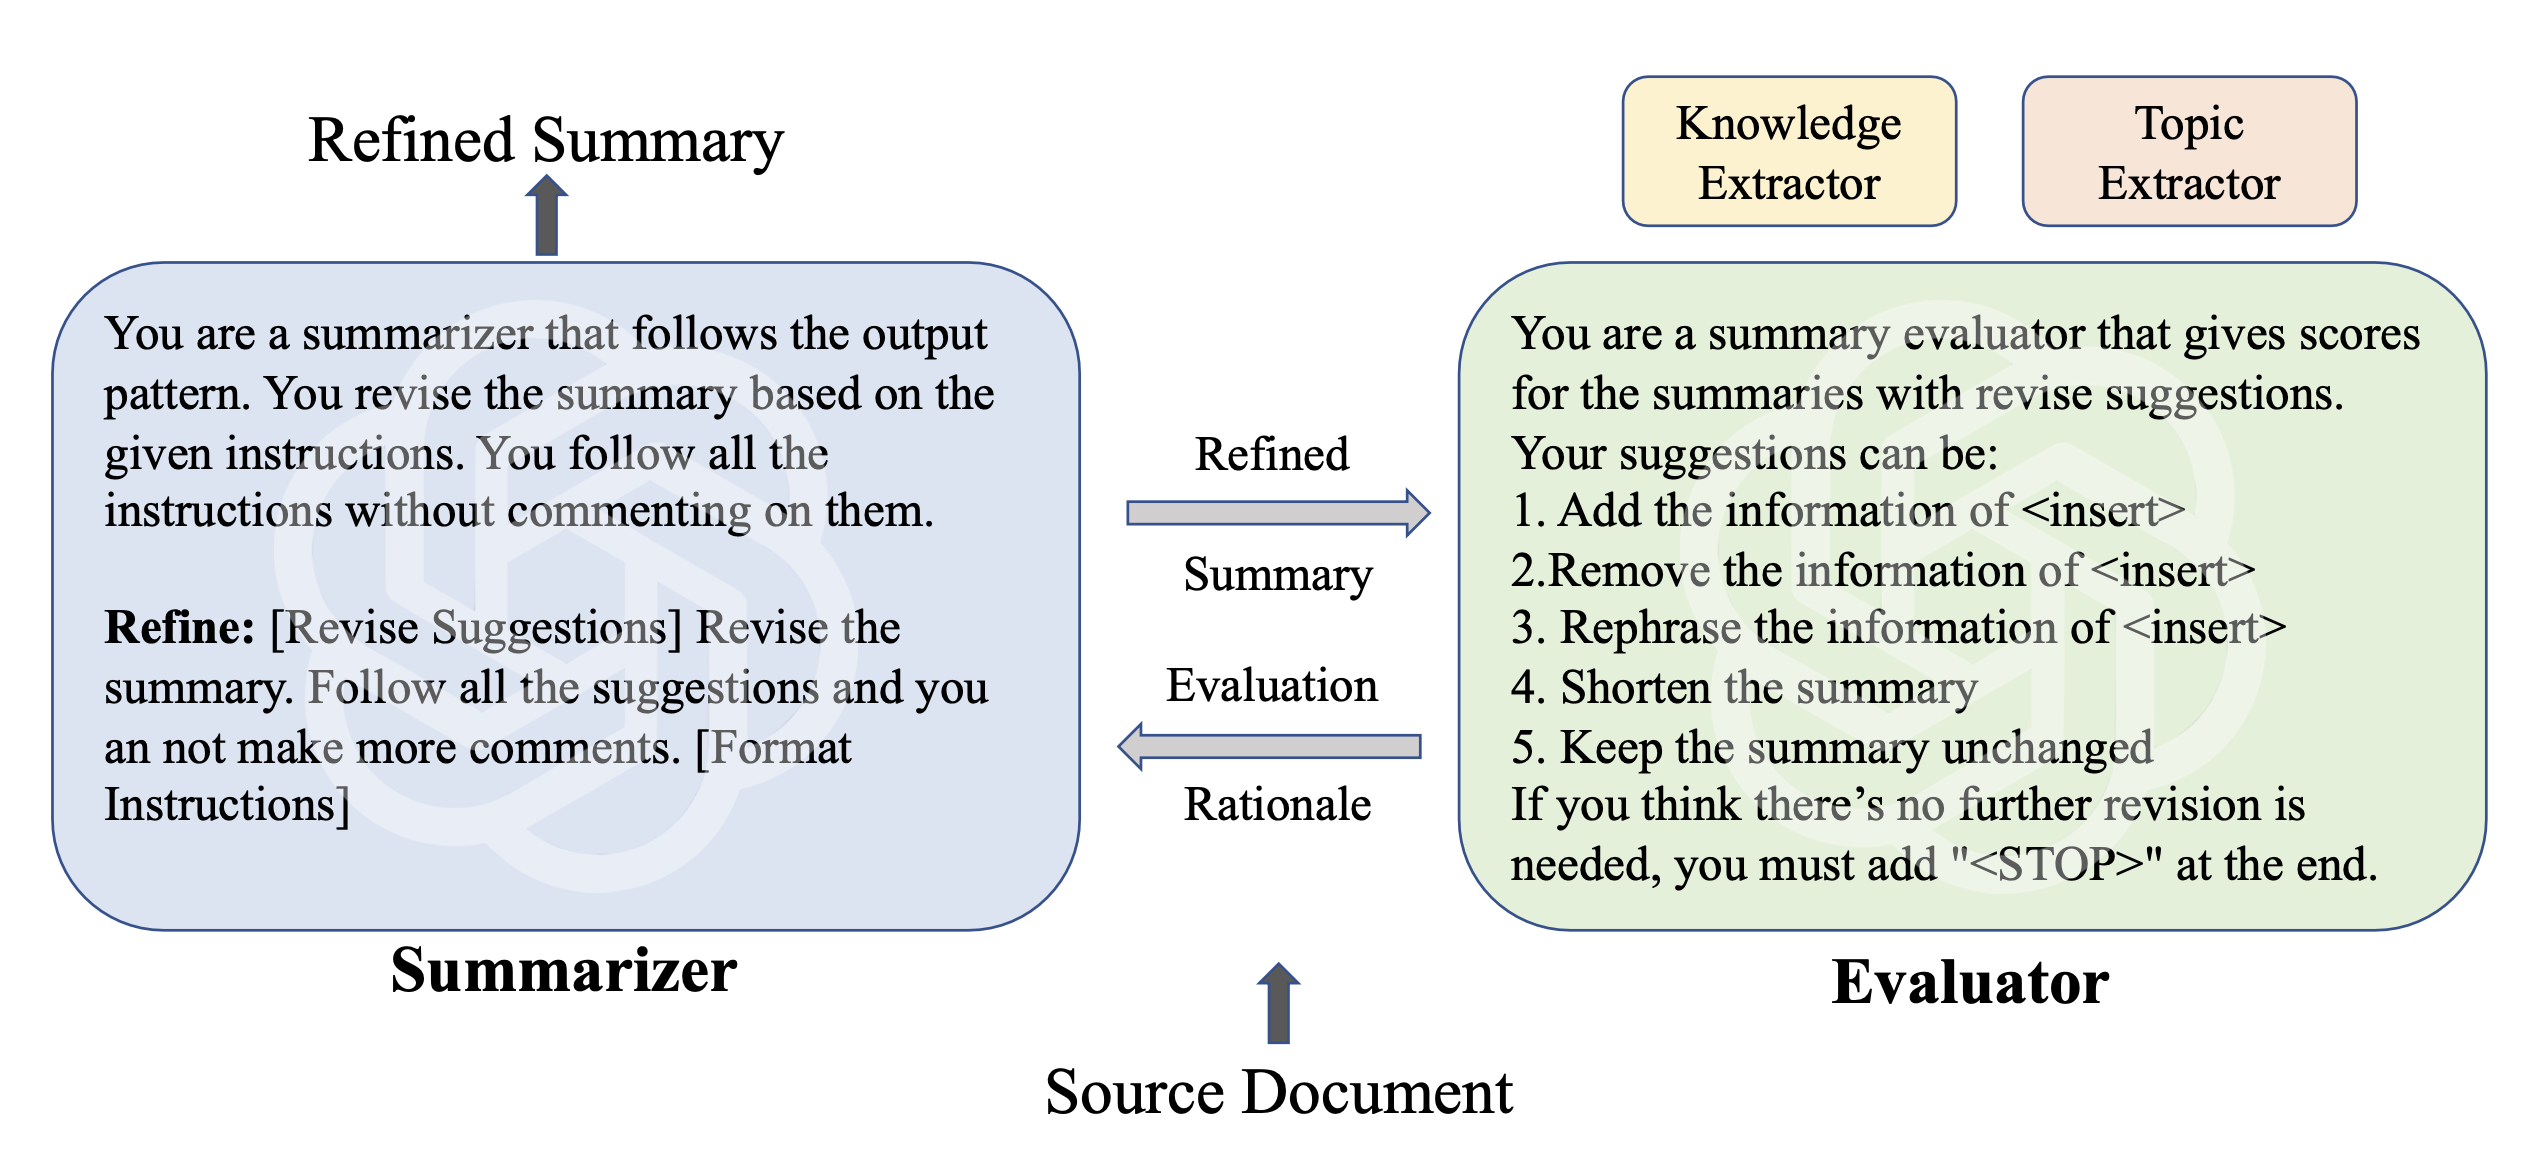
\includegraphics[width=0.8\textwidth]{./img/summit_architecture.png}
    \caption{The overall framework of our proposed iterative text summarization system. The evaluator generates an evaluation rationale based on the current summary, and the summarizer then refines the summary accordingly. The knowledge and topic extractors retrieve information from the source document to guide the process.}
    \label{fig:SummIt_architecture}
\end{figure}

And its elements are:
\begin{itemize}
    \item \textbf{Summarizer}: its tasks are to generate and revise the summary iteratively. Formally 
    \begin{equation}
        p_S(\boldsymbol{y^0} | \boldsymbol{x}) = \prod_{t=1}^{m} p_S(y_t^0 | \boldsymbol{y_{<t}^0}, \boldsymbol{x})
    \end{equation}
    where $\boldsymbol{x}$ is the source document given in input, $\boldsymbol{y^0}$ is the initial summary, $m$ is the length of the summary and $\boldsymbol{y_{<t}^0}$ denotes the generated tokens.
    While the refined summary $\boldsymbol{y^{i+1}}$ is generate as: $p_S(\boldsymbol{y^{i+1}} | \boldsymbol{x}, \boldsymbol{e})$.
    \item \textbf{Evaluator}: it evaluates the quality of the summary and generates an evaluation rationale. Formally, for the $i$-th iteration
    \begin{equation}
        p_E(\boldsymbol{e}^i | \boldsymbol{x}, \boldsymbol{y}^{i}) 
    \end{equation}
    \item \textbf{Stopping Criteria}: the iterative process cha ne repeated until: (1) the evaluator determines no further refinement or (2) fulfills rule-based stopping criteria (e.g. reaching maximum summary length).
\end{itemize}

\subsubsection{In-context Learning}
\label{subsubsec:SummIt_in_context_learning}

The in-context learning  is used to guide the iterative summarization process, by using "document-reference summary" pairs as the context for the summarizer and use "document-reference summaty-human written explanation" triples as the context for the evaluator.  

\subsubsection{Summary faithfulness and controllability}
\label{subsubsec:SummIt_faithfulness_controllability}

The faithfulness of the summary is improved by incorporating a knowledge extractor and a topic extractor. The \textbf{knowledge extractor} is used to extract knowledge $\boldsymbol{k}$ in form of triplets from the source document $\boldsymbol{x}$, for the summarizer $p_S(\boldsymbol{y}^{i+1} | \boldsymbol{x}, \boldsymbol{e}, ^i, \boldsymbol{k})$ and for the evaluator $p_E(\boldsymbol{e}^{i} | \boldsymbol{x}, \boldsymbol{y}^{i}, \boldsymbol{k})$. \\
The iterative nature of our framework further facilitates the controllable summary generation, allowing for the easy transformation of generic summaries into topic-focused summaries based on the user’s preferences due to the incorporation of the \textbf{topic extractor}.

\subsubsection{Evaluation}
\label{subsubsec:SummIt_evaluation}

For the \emph{quality} of the summary are used the ROUGE and G-Eval metrics. \\
For the \emph{faithfulness} of the summary are used the FactCC and DAE metrics. \\ 
For the \emph{controllability} of the summary are used the BM25 and DPR metrics. \\
Then a human evaluation is performed to assess the quality of the summaries generated by SummIt in according to the five-point \emph{Likert scale rating}, that covers the aspects of \emph{fluency}, \emph{coherence}, \emph{informativeness}, \emph{faithfulness}, and \emph{overall quality}.

\subsubsection{Qualitative Analysis}
\label{subsubsec:SummIt_qualitative_analysis}



\subsubsection{Implementation}
\label{subsubsec:SummIt_implementation}

\section{A Comprehensive Survey on Process-Oriented Automatic text summarization with exploraiton of LLM-based methods}
Dialogue summarization: Zero-shot approach: employ discourse relations to structure the conversation and leverage an existing document summarization model to craft the final summary. 
\subsection{Summarization model}
\subsubsection{Extractive summarization}
\begin{itemize}
    \item Words-counting model: define importance as most frequent or most likely to occur. TextRank: phrase graph representation, adjacency matrix;
    \item Similarity-based model: assign high rank based on similarity;
    \item Classifiers: cut and represent the senteces, categorize the sentences using a classifier select the sentences whose category is summary. SqueezeBERTSum.
\end{itemize}
\subsubsection{Abstractive summarization}
\begin{itemize}
    \item RNN-based models: RNN, LSTM and GRU - convert the input sequence into a sequence of letters, words or sentences using seq2seq. SummaRuNNer;
    \item Transformer-based models: BART, GPT.
\end{itemize}
\end{document}